\documentclass[9pt]{article}

% packages
\usepackage[utf8]{inputenc}
\usepackage[english]{babel}
\usepackage{bm}
\usepackage[a4paper]{geometry}
\usepackage{graphicx}
\graphicspath{{./images/}}
\usepackage[font=small,labelfont=bf]{caption}
\usepackage{subcaption}
\usepackage{amsthm}
\usepackage{amsmath}
\usepackage{amsfonts}
\usepackage{enumitem}
\usepackage{mathtools}
\usepackage{commath}
\usepackage[ruled,vlined]{algorithm2e}

\theoremstyle{definition}
\newtheorem{definition}{Definition}[section]
\newtheorem{theorem}{Theorem}[section]
\newtheorem{proposition}{Proposition}[section]
\newtheorem*{note}{Note}
\newtheorem*{remark}{Remark}
\newtheorem*{observation}{Observation}

%opening
\title{Elliptic Curve Cryptography}
\author{Cieno Marco, Viviani Ivan}
\date{}

\begin{document}

\maketitle
\thispagestyle{empty}
\begin{abstract}
Elliptic Curve Cryptography (ECC) is an approach to public key cryptography based on the algebraic structure of elliptic curves over finite fields.

Elliptic curves allow for key agreement protocols, digital signatures, pseudorandom number generators, and other tasks. Indirectly, they can be used for encryption by combining the key agreement with symmetric encryption schemes.

The well--known Diffie--Hellman and ElGamal schemes can both be efficiently implemented with elliptic curves, without any substantial change, and provide equivalent levels of security with smaller keys compared to their non--elliptic counterparts. On the wave of ECC, the field of pairing--based cryptography recently exploded. Elliptic curve pairings allow creating many interesting cryptographic schemes with real--world applications, some of which are identity--based cryptography and non--interactive zero--knowledge proofs (NIZKP).
\end{abstract}

%%%%%%%%%%%%%%%%%%%%%%%%%%%%%%%%%%%%%%%%%%%%%%%%%
% Just a fancy way to get page numbers properly %
%%%%%%%%%%%%%%%%%%%%%%%%%%%%%%%%%%%%%%%%%%%%%%%%%
\clearpage %%%%%%%%%%%%%%%%%%%%%%%%%%%%%%%%%%%%%%
\tableofcontents %%%%%%%%%%%%%%%%%%%%%%%%%%%%%%%%
\setcounter{page}{1} %%%%%%%%%%%%%%%%%%%%%%%%%%%%
\renewcommand{\thepage}{\textsc{\roman{page}}} %%
\clearpage %%%%%%%%%%%%%%%%%%%%%%%%%%%%%%%%%%%%%%
\setcounter{page}{1} %%%%%%%%%%%%%%%%%%%%%%%%%%%%
\renewcommand{\thepage}{\arabic{page}} %%%%%%%%%%
%%%%%%%%%%%%%%%%%%%%%%%%%%%%%%%%%%%%%%%%%%%%%%%%%


\section{Evolution of public key cryptography}
The idea of a public key cryptosystem was first introduced by Whitfield Diffie and Martin Hellman in the late 1970s. They proposed a paradigm in which two different but mathematically related keys are used -- a public key and a private key.
The RSA cryptosystem was shortly after invented and patented by Ron Rivest, Adi Shamir, and Leonard Adleman. 
Being the only public key cryptosystem at the time, it immediately caught the attention of the academic community which helped to validate its security, giving visibility to the integer factorization problem.

Elliptic curves were first introduced to the cryptographic community in 1984 when Hendrik Lenstra proposed a new factorization method based on such a mathematical object. In 1985, Neal Koblitz and Victor S. Miller independently proposed to use elliptic curves to create cryptosystems under the suggestion that the problem associated with them might be more difficult than the classical discrete logarithm problem (DLP) on finite fields, though it was hard to confirm with any confidence since at the time there was no active research on the former problem. In the same year, the invention of the ElGamal public key cryptosystem provided a royalty--free alternative to RSA. A major dilemma pervading the field of cryptography is that no one knows the actual difficulty of the supposedly hard problems on which it is based. Currently, the security of public key cryptosystems depends on the perception and consensus of experts as to the difficulty of problems such as integer
factorization and discrete logarithms. Serious study of the elliptic curve discrete logarithm problem (ECDLP) started in the late 1980s and more than a decade after its introduction the security of ECC was still questioned by leading experts.

Time went by and, in the early 2000s, the NSA made elliptic curve its standard suite B algorithm for both encryption and signature. Nowadays elliptic curves are suggested by the Commercial National Security Algorithm Suite and their use on low power devices has been shown to be much more scalable than RSA.

\section{Elliptic curves}

Generally speaking, an elliptic curve is the set of solutions to an equation of the form $Y^2 = X^3 + AX + B$.

One important feature of elliptic curves, that allowed for their application to public key cryptography, is the fact that there is a natural way of performing the ``addition" of two points on the curve to obtain a third point on the same curve. We refer to this operation as \textit{addition law} since it is analogous to integer addition in some aspects, but keep in mind that it is still very unlike it.

\begin{remark}
The addition law does not work well on elliptic curves that have singular points (\textit{i.e.}, curves with cusps or self--intersections). Hence, we require the curve to be non--singular, which happens if and only if the cubic polynomial $X^3 + AX + B$ has no repeated roots.
\end{remark}

\begin{definition}[Elliptic curve]
An \textit{elliptic curve} $E$ is the set of solutions to a Weierstrass equation
$$E \, : \, Y^2 = X^3 + AX + B,$$
where the discriminant is
$$\Delta_E = -16 \left( 4 A^3 + 27 B^2 \right) \neq 0,$$
together with a point $\mathcal{O}$ at infinity.
\end{definition}

\begin{figure}[h]
	\centering
	\begin{subfigure}[b]{0.35\textwidth}
		\centering
		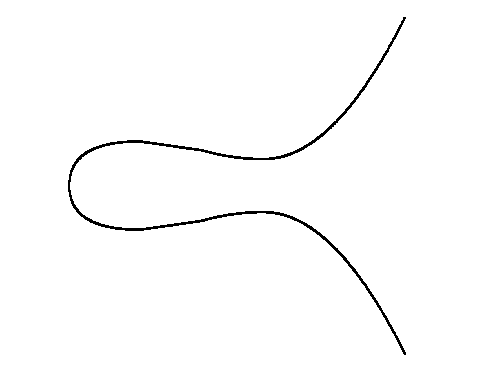
\includegraphics[width=\textwidth]{exEC1.png}
		\caption{$Y^2 = X^3 - 3X + 3$}
		\label{fig:ec1}
	\end{subfigure}
	\begin{subfigure}[b]{0.35\textwidth}
		\centering
		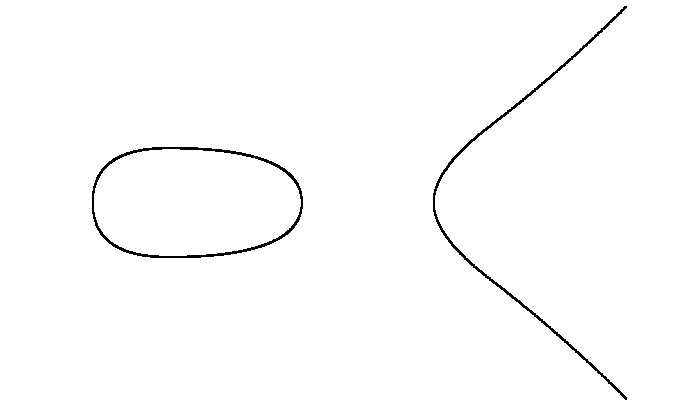
\includegraphics[width=\textwidth]{exEC2.png}
		\caption{$Y^2 = X^3 - 6X + 5$}
		\label{fig:ec2}
	\end{subfigure}
	\caption{Two examples of elliptic curves.}
	\label{fig:2ec}
\end{figure}

\subsection{Addition law on elliptic curves}
Now that we know what elliptic curves look like, we proceed to describe the \textit{addition law} using a geometrical approach, a graphic representation of which is shown in Figure~\ref{fig:addlaw}. This will be enough for us to provide a formal definition of \textit{elliptic curve}. Then we will develop explicit formulas for adding two points of an elliptic curve in the form of an ``addition algorithm".

\begin{figure}[h]
	\centering
	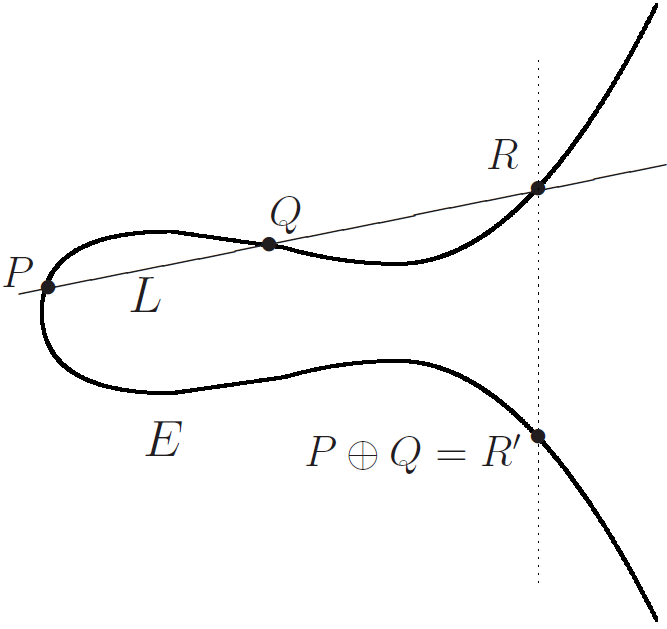
\includegraphics[width=0.4\textwidth]{addlaw.png}
	\caption{Graphical representation of two points addition on an elliptic curve.}
	\label{fig:addlaw}
\end{figure}

Given two points $P$ and $Q$ on an elliptic curve $E$, we first draw the line $L$ through them, which also intersects $E$ at a third point $R$. Then we leverage the symmetry of the curve about the $X$--axis and get the point $R'$, \textit{i.e.}, the reflection of $R$ across the $X$--axis. The point $R'$ is called the ``sum of $P$ and $Q$", denoted by $R' = P \oplus Q$. The mathematical implementation of these steps is rather trivial: for further details refer to \cite[Example~5.1]{JH08}.

The addition law for two distinct and not vertically aligned points works fine, but we still need to cover two edge cases: adding a point to itself and to its reflection about the $X$--axis.

\paragraph{Adding $P$ to itself}
In this case, the line $L$ simply becomes the tangent line to $E$ at $P$ and still intersects $E$ at another point $R$, so we can proceed as before except for determining the equation of $L$: for further details refer to \cite[Example~5.2]{JH08}.

\paragraph{Adding $P$ to its reflection}
In this case, the line $L$ through $P = (x_P, y_P)$ and $P' = \ominus P = (x_P, -y_P)$ is the vertical line $L: X = x_P$ which does not intersect $E$ at any other point. This is why we also included the extra point $\mathcal{O}$, which does not exist in the $XY$--plane and lives ``at infinity". We pretend that it lies on every vertical line, so we can write $P \oplus P' = \mathcal{O}$.

It may appear as though adding $\mathcal{O}$ to an ordinary point $P$ could rise an issue, but simply applying the general procedure leads us back to the point $P$ itself, so we can write $P \oplus \mathcal{O} = P$.

\begin{note}
For the sake of simplicity we'll denote addition as $+$ and reflection as $-$, so $P - Q = P + (-Q) = P \oplus (\ominus Q)$. We further represent repeated addition as multiplication of a point by an integer: $\underbrace{P + P + \cdots + P}_{n\text{ times}} = nP.$
\end{note}

\begin{figure}[h]
	\centering
	\begin{subfigure}[b]{0.4\textwidth}
		\centering
		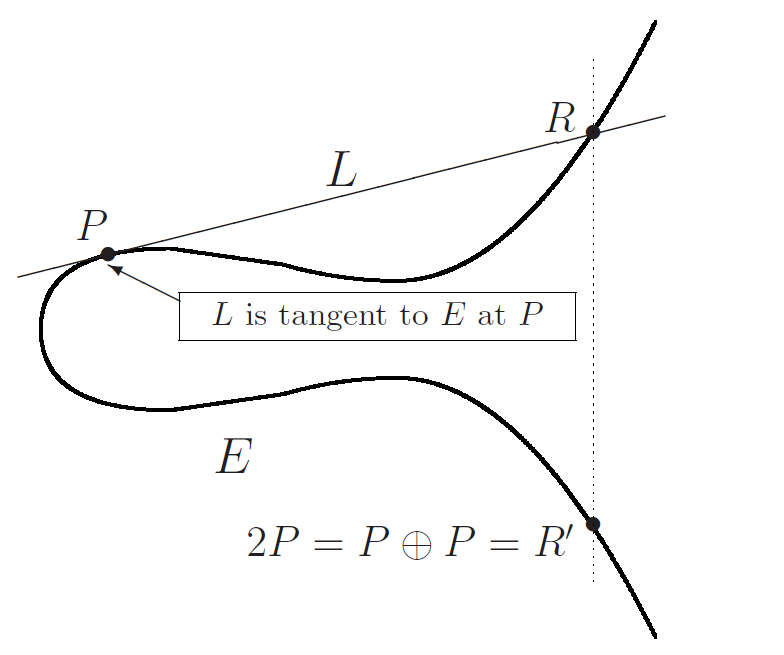
\includegraphics[width=1.17\textwidth]{addPtoP.png}
		\caption{Adding a point $P$ to itself.}
		\label{fig:addPtoP}
	\end{subfigure}
	%\hfill
	\begin{subfigure}[b]{0.4\textwidth}
		\centering
		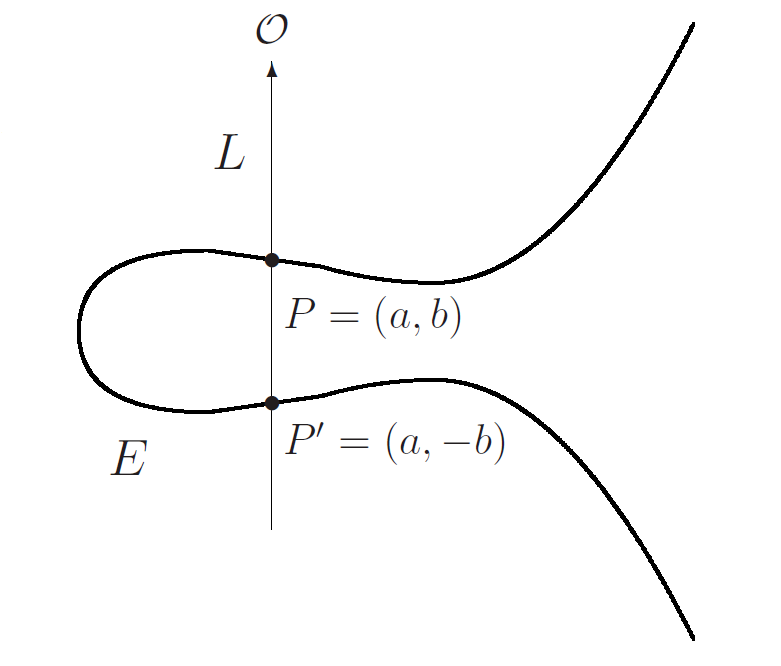
\includegraphics[width=1.15\textwidth]{addPto-P.png}
		\caption{Adding a point $P$ to $P' = -P$.}
		\label{fig:addPto-P}
	\end{subfigure}
	\hfill
	\caption{Edge cases of the addition law.}
	\label{fig:2cases}
\end{figure}

\begin{theorem}[\textit{Properties of the addition law}]
The addition law makes the points of $E$ into an abelian group. That is, $\forall P,Q,R \in E$, the following properties hold.
\begin{enumerate}[label=(\alph*)]
	\item $P + \mathcal{O} = \mathcal{O} + P = P$ \hfill [Identity]
	\item $P + (-P) = \mathcal{O}$ \hfill [Inverse]
	\item $(P + Q) + R = P + (Q + R)$ \hfill [Associative]
	\item $P + Q = Q + P$ \hfill [Commutative]
\end{enumerate}
\label{th:propaddlaw}
\end{theorem}
\begin{proof}
	The fact that $\mathcal{O}$ lies on all vertical lines proves the identity and inverse properties (a) and (b). Proving the commutative property (d) is trivial, while the associative property (c) is rather hard to prove. After we develop explicit formulas for the addition law on $E$, one can use them to check (c) by direct calculation, but more elegant proofs can be found in the literature.
\end{proof}

\subsection{Elliptic Curve Addition Algorithm (ECAA)}
To easily add and subtract points on an elliptic curve, we need to find explicit formulas, which we provide in the form of an algorithm called \textit{Elliptic curve addition algorithm} (ECAA). The pseudocode of ECAA is shown in Algorithm~\ref{alg:ECAA}.

\begin{theorem}[\textit{Elliptic curve addition algorithm}]
	Let $E \, : \, Y^2 = X^3 + AX + B$ be an elliptic curve and let $P_1$ and $P_2$ be two points on $E$.
	\begin{enumerate}[label=(\alph*)]
		\item If $P_1 = \mathcal{O}$, then $P_1 + P_2 = P_2$
		\item Otherwise, if $P_2 = \mathcal{O}$, then $P_1 + P_2 = P_1$
		\item Otherwise, write $P_1 = (x_1, y_1)$ and $P_2 = (x_2, y_2)$
		\item If $x_1 = x_2$ and $y_1 = -y_2$, then $P_1 + P_2 = \mathcal{O}$
		\item Otherwise define $\lambda$ by
			  \begin{align*}
			  	\lambda = 
			  	\begin{cases*}
			  		\dfrac{y_2 - y_1}{x_2 - x_1}, \;\; \text{if} \;\; P_1 \neq P_2\\
			  		\dfrac{3x_1^2 + A}{2y_1}, \;\; \text{if} \;\; P_1 = P_2
			  	\end{cases*}
			  \end{align*}
			  and let $x_3 = \lambda^2 - x_1 - x_2$ and $y_3 = \lambda(x_1 - x_3) - y_1$. Then $P_1 + P_2 = (x_3, y_3).$
	\end{enumerate}
    \label{th:ecaa}
\end{theorem}
\begin{proof}
	In parts (a) and (b) we check whether one of the two points on $E$ is equal to $\mathcal{O}$, and in (d) we check whether they are opposites. In part (e), if $P_1 \neq P_2$ then $\lambda$ is the slope of the line $L$ through $P_1$ and $P_2$, otherwise if $P_1 = P_2$ then $\lambda$ is the slope of the tangent line at $P_1 = P_2$. In either case $L \, : \, Y = \lambda X + \nu$ with $\nu = y_1 - \lambda x_1$. Substituting the equation for $L$ into the equation for $E$ gives the polynomial $P(X) = X^3 - \lambda^2 X^2 + (A - 2\lambda\nu)X + (B - \nu^2)^2 = 0$. The roots of this cubic are $x_1$, $x_2$ (which are known), and we call the third $x_3$, so we can write $P(X) = (X - x_1)(X - x_2)(X - x_3)$. Multiplying out the right--hand side and comparing the coefficients of $X^2$ on each side gives $x_3 = \lambda^2 - x_1 - x_2$. We eventually obtain the $Y$--coordinate of $P_1 + P_2$ by solving $-y_3 = \lambda x_3 + \nu$.
\end{proof}

\begin{algorithm}[h]
	\SetAlgoLined
	\textbf{Input}: $E \, : \, Y^2 = X^3 + AX + B$, $P_1 \in E$, $P_2 \in E$ \\
	\textbf{Output}: $P_1 + P_2$ \\ 
	\lIf{$P_1 = \mathcal{O}$}{\Return $P_2$}
	\lIf{$P_2 = \mathcal{O}$}{\Return $P_1$}
	$P_1 \gets (x_1, y_1)$; $P_2 \gets (x_2, y_2)$; \\
	\lIf{$x_1 = x_2 \, \wedge \, y_1 = -y_2$}{\Return $\mathcal{O}$}
	\eIf{$P_1 \neq P_2$}{$\lambda \gets \frac{y_2 - y_1}{x_2 - x_1}$;}{$\lambda \gets \frac{3x_1^2 + A}{2y_1}$;}
	$x_3 \gets \lambda^2 - x_1 - x_2$; $y_3 \gets \lambda(x_1 - x_3) - y_1$; \\
	\Return $(x_3, y_3)$
	\caption{Elliptic curve addition algorithm (ECAA)}
	\label{alg:ECAA}
\end{algorithm}

\clearpage\section{Elliptic curves over finite fields}

In the previous section we introduced the theory of elliptic curves geometrically. However, in order to apply it to cryptography, we need to look at elliptic curves whose points have coordinates in a finite field $\mathbb{F}_p$.

\begin{definition}[Elliptic curve over a finite field]
    Let $\mathbb{F}_p$ be a finite field of characteristic $p \geq 3$. An \textit{elliptic curve over $\mathbb{F}_p$}, denoted by $E/\mathbb{F}_p$, is the set of solutions to a Weierstrass equation
	$$E \, : \, Y^2 = X^3 + AX + B \qquad \text{with $A, B \in \mathbb{F}_p$ satisfying $\Delta \not\equiv 0$}.$$
	
	We further denote the set of points on $E$ with coordinates in $\mathbb{F}_p$ by 
	$$E(\mathbb{F}_p) = \{(x, y) : x, y \in \mathbb{F}_p \wedge y^2 = x^3 + Ax + B\} \cup \{\mathcal{O}\}.$$
\end{definition}

\begin{remark}
    We require $p \geq 3$ because, given any elliptic curve $E$, the set $E(\mathbb{F}_2)$ consists of at most 5 points, so it's not useful in cryptography. However, the binary nature of computers tends to make them operate more efficiently in situations in which $2 = 0$. This happens in $\mathbb{F}_2$, as well as in its, so--called, \textit{extension fields} $\mathbb{F}_{2^k}$.
    
    In a nutshell, elements of extension fields $\mathbb{F}_{p^k}$ are usually represented as polynomials $a_0 + a_1 x + \dots + a_{k-1} x^{k-1}$ and computations are achieved by performing polynomial addition and convolution. Elliptic curves over $\mathbb{F}_{p^k}$ are defined by generalized Weierstrass equations, $E: Y^2 + a_1 XY + a_3 Y = X^3 + a_2 X^2 + a_4 X + a_6$. Geometrically speaking, the addition law remains almost untouched, although the ECAA should be modified because slope and intersections have different formulations than before. The key to efficiency lies in a suggestion of Neal Koblitz, that using an elliptic curve $E/\mathbb{F}_2$ while taking points on $E(\mathbb{F}_{2^k})$, allows the use of the \textit{$p$--power Frobenius map}
    \begin{align*}
        \tau : \mathbb{F}_{p^k} &\longrightarrow \mathbb{F}_{p^k}\\
               \alpha &\longmapsto \alpha^p,
    \end{align*}
    in place of the \textit{doubling map}, later described in Section~\ref{sec:double-and-add}.
    
    We refer the reader to \cite[Section~5.7]{JH08} for an introduction and to any standard text on elliptic curves for a complete understanding of this topic.
\end{remark}

\subsection{Addition Law (revisited) and the set $E(\mathbb{F}_p)$}
Given an elliptic curve $E$ and a finite field $\mathbb{F}_p$, we can find the points of $E(\mathbb{F}_p)$ by substituting in all possible values of $X$, \textit{i.e.}, $\{0,1,2,...,p-1\}$, and checking for which values the quantity $X^3 + AX + B$ is a square modulo $p$. For further details refer to \cite[Example~5.8]{JH08}.

For brevity of exposition, we use the explicit formulas given in Theorem~\ref{th:ecaa} to add points in $E(\mathbb{F}_p)$, but note that we could develop a theory of geometry using the field $\mathbb{F}_p$ instead of $\mathbb{R}$ and mimic our earlier constructions to define the sum of two points: this leads to the field of mathematics called \textit{algebraic geometry}.

\begin{observation}
	The only operations used in ECAA are addition, subtraction, multiplication, and division involving the coefficients of $E$ and the coordinates of $P$ and $Q$. Since all of those are in the field $\mathbb{F}_p$, the coordinates of the resulting point are in $\mathbb{F}_p$.
\end{observation}

\begin{theorem}[\textit{Addition in $E/\mathbb{F}_p$}]
	Given an elliptic curve $E$ over a finite field $\mathbb{F}_p$ and two points $P, Q \in E(\mathbb{F}_p)$:
	\begin{enumerate}[label=(\alph*)]
		\item ECAA (Algorithm~\ref{alg:ECAA}) applied to $P$ and $Q$ yields a point $P + Q \in E(\mathbb{F}_p)$.
		\item This \textit{addition law} on $E(\mathbb{F}_p)$ makes $E(\mathbb{F}_p)$ into a finite group.
	\end{enumerate}
\end{theorem}
\begin{proof}
	The derivation of the formulas in Theorem~\ref{th:ecaa}(e) shows why part (a) is true, although when $P = Q$ we also need to indicate why the resulting cubic polynomial has a double root. For part (b) we need to show that the properties of Theorem~\ref{th:propaddlaw} hold. The identity law, inverse law, and commutative law follow from considerations on the steps of ECAA (Theorem~\ref{th:ecaa}); while the associative law is not so clear and to prove it we would need to develop more of the general theory of elliptic curves, thus refer to the literature.
\end{proof}

It is clear the set $E(\mathbb{F}_p)$ is a finite set, since there are only $p$ possible $X$--coordinates, each with at most two corresponding $Y$--coordinates. This estimate provides a very loose bound. An exact formula to calculate the cardinality $\#E(\mathbb{F}_p)$ is given by \textit{Hasse's theorem}, for which we refer the reader to \cite[Theorem~5.11]{JH08}. An immediate consequence of this theorem is the (tight) bound
$$(\sqrt{p} - 1)^2 \leq \#E(\mathbb{F}_p) \leq (\sqrt{p} + 1)^2.$$
This suggests that the set $E(\mathbb{F}_p)$ always contains about $p$ points, so for big enough primes it could be suitable for cryptographic applications.


\section{Elliptic Curve Discrete Logarithm Problem (ECDLP)}
In this section we are going to talk about the difficult problem on which ECC is built, deriving it from the \textit{discrete logarithm problem} (DLP) in the finite field $\mathbb{F}_p^\ast$, used in ``classical" cryptography, by analogy.

In order to create a cryptosystem based on the DLP for $\mathbb{F}_p^\ast$, Alice chooses $g \in \mathbb{F}_p^\ast$ and a secret integer $\alpha$. She calculates $h \equiv g^\alpha \pmod{p}$ and publishes $g$ and $h$. An adversary who is willing to recover the secret $\alpha$ needs to figure out how many times $g$ must be multiplied by itself to obtain $h$. This problem is thought to be hard enough.

In an analogous way, Alice could choose a point $P \in E(\mathbb{F}_p)$ and a secret integer $\alpha$ and publish $P$ and $Q = \alpha P$. This elliptic analogue of the DLP is thought to be even more difficult to solve than the original one, mainly because addition on $E$ is a complicated operation.

\begin{definition}[ECDLP]
	Given an elliptic curve $E$ over $\mathbb{F}_p$ and two points $P, Q \in E(\mathbb{F}_p)$, the \textit{Elliptic Curve Discrete Logarithm Problem} (ECDLP) is the problem of finding an integer $n$ such that $Q = n P$. By analogy with the DLP for $\mathbb{F}_p^\ast$, the integer $n$ is called \textit{elliptic discrete logarithm of Q with respect to P} and is denoted by $n = \log_P(Q)$.
\end{definition}

\begin{remark}
	The definition of $\log_P(Q)$ provided is not precise for two reasons:
	\begin{enumerate}
		\item There may be points $P$,$Q \in E(\mathbb{F}_p)$ such that $Q$ is not a multiple of $P$. In this case $\log_P(Q)$ is undefined.
		\item If there is one value of $n$ such that $Q = n P$, then there are many such values.
	\end{enumerate}
\end{remark}

In practice, Alice starts out with a public point $P$ and a secret integer $n$ and then computes $Q = n P$, so (1) is never the case. To better understand (2), we first provide the following proposition.

\begin{proposition}
	$\forall P \in E(\mathbb{F}_p) \;\; \exists s \in \mathbb{Z}^+ : sP = \mathcal{O}$.
\end{proposition}

\begin{proof}
	Since $E(\mathbb{F}_p)$ is finite, the points in the list $P,\,2P,\,3P,\,\dots$ cannot all be distinct, \textit{i.e.}, $\exists k,j \in \mathbb{Z}^+, k > j : k P = j P$. We can take $s = k - j$.
\end{proof}

The smallest such integer, $\bar{s} = \min\{s > 0 : s P = \mathcal{O}\}$, is called the \textit{order of} $P$. Lagrange's theorem tells us that $\bar{s}$ divides $\#E(\mathbb{F}_p)$, thus given $\bar{s}$ and any integer $n_0$ such that $Q = n_0P$, the solutions to $Q = n P$ are the integers $n = n_0 + i\bar{s} \;\; \forall i \in \mathbb{Z}$. In other words, $\log_P(Q)$ is an element of $\mathbb{Z}/\bar{s}\mathbb{Z}$ and the following property holds:
$$\log_P(Q_1 + Q_2) = \log_P(Q_1) + \log_P(Q_2) \qquad \forall Q_1,Q_2 \in E(\mathbb{F}_p).$$

Therefore the discrete logarithm for $E(\mathbb{F}_p)$ respects the addition law when the group $E(\mathbb{F}_p)$ is mapped to the group $\mathbb{Z}/\bar{s}\mathbb{Z}$. We say that the map $\log_P$ defines a \textit{group homomorphism}
\begin{align*}
	\log_P : E(\mathbb{F}_p) \longrightarrow \mathbb{Z}/\bar{s}\mathbb{Z}.
\end{align*}

For details about the calculation of the discrete logarithm for $E(\mathbb{F}_p)$ refer to \cite[Example~5.15]{JH08}.

\subsection{Double--and--Add Algorithm}\label{sec:double-and-add}
Any cryptosystem based on elliptic curves requires the calculation of $Q = n P$. This can be done efficiently with a procedure that is analogous to the \textit{square--and--multiply} algorithm for modular exponentiation. The algorithm is called \textit{double--and--add} and it comprises the following steps:
\begin{enumerate}
	\item We write $n$ in binary form:
	\begin{align*}
		n = \sum_{j = 0}^{r}n_j 2^j \qquad \text{where } n_j \in \{0,1\} \wedge n_r = 1.
	\end{align*}
	\item We compute the 2-power multiples of $P$:
	\begin{align*}
	    Q_0 = P, \quad Q_1 = 2P, \quad \dots, \quad Q_i = 2^i P, \quad \dots, \quad Q_r = 2^r P
	\end{align*}
	This step requires $r$ doublings, since $Q_0 = P \;\; \wedge \;\; Q_i = 2 Q_{i-1}$.
	\item  We compute $n P$ using at most $r$ additional additions, thus at most $2r$ operations in total:
	\begin{align*}
		Q = n P = \sum_{i = 0}^{r}n_i Q_i.
	\end{align*}
\end{enumerate}

Notice that $n \geq 2^r \Longrightarrow 2r \leq 2\log_2(n)$, so computing $n P$ is feasible even for very large values of $n$. The pseudocode of the Double--and--Add Algorithm is shown in Algorithm~\ref{alg:DAA}.

\begin{algorithm}[H]
	\SetAlgoLined
	\textbf{Input}: point $P \in E(\mathbb{F}_p)$, integer $n \geq 1$ \\
	\textbf{Output}: point $n P$ \\ 
	$Q \gets P$; $R \gets \mathcal{O}$; \\
	\While{$n > 0$}{
		\lIf{$n \equiv 1 \pmod{2}$}{$R \gets R + Q$}
		$Q \gets 2Q$;\\
		$n \gets \lfloor n/2 \rfloor$; \\
	}
	\Return $R$
	\caption{Double--and--Add Algorithm}
	\label{alg:DAA}
\end{algorithm}

\begin{observation}
    The number of point operations is at most $2r + 1$, where $r$ is the exponent of the largest power of $2$ that appears in the binary expansion of $n$. If we could write $n$ as a sum of fewer terms, we could save some operations. This can be achieved by writing $n$ as sums and differences of powers of $2$ (ternary expansion):
    \begin{align*}
        n = \sum_{i = 0}^{k}u_i 2^i \qquad \text{where } u_i \in \{-1,0,1\} \wedge k = \lfloor\log_2(n)\rfloor+1.
    \end{align*}
    
    By allowing ternary expansions one can show that computing $nP$ never requires more than $\frac{3}{2}k + 1$ point operations ($k + 1$ doublings and $\frac{1}{2}k$ additions), with most instances requiring about $\frac{4}{3}k + 1$ operations.
    % saltata Proposition 5.18
\end{observation}

\subsection{How hard is the ECDLP?}
In literature there are algorithms that solve the ECDLP for $E(\mathbb{F}_p)$ in $O(\sqrt{p})$ steps. The DLP for $\mathbb{F}_p^\ast$, instead, can be solved faster by an index calculus algorithm that runs in sub--exponential time.
Although instances that are easy to solve exist for both problems, there are no index calculus algorithms known for the ECDLP, making it look like it is much more difficult than the DLP. This is the main reason why elliptic curves are now suggested in cryptography.

\section{Elliptic Curve Cryptography}
We are ready to apply elliptic curves to cryptography. In particular, we are going to describe the elliptic analogues of the Diffie--Hellman key exchange and the ElGamal public key cryptosystem.

\subsection{Elliptic curve Diffie--Hellman key exchange}
To construct the elliptic analogue of the Diffie--Hellman key exchange we only need to replace the DLP for $\mathbb{F}_p$ with the ECDLP for $E(\mathbb{F}_p)$ and make minor adjustments. Intuitively, we will compute and exchange points of an elliptic curve on a finite field instead of numbers in a finite field. Note that in practice, since the coordinates of any point of an elliptic curve are related by its (public) formula, the shared secret key can depend only on the $X$--coordinate. The steps are the following:
\begin{enumerate}[label=\textbf{\arabic*.}]
    \item \textbf{Public parameter creation}: a trusted third party publishes a large prime number $p$, an elliptic curve $E$ and a point $P \in E(\mathbb{F}_p)$. 
    \item \textbf{Private computations}:
        \begin{itemize}
            \item Alice chooses a secret integer $n_A$ and computes the point $Q_A = n_A P$.
            \item Bob chooses a secret integer $n_B$ and computes the point $Q_B = n_B P$.
        \end{itemize}
    \item \textbf{Public exchange of values}: Alice and Bob exchange the $X$--coordinates of $Q_A$ and $Q_B$.
    \item \textbf{Further private computations}: Alice and Bob each compute one of the points $\pm n_A Q_B = \pm n_B Q_A = \pm n_A n_BP$ by "guessing" one of the two possible $Y$--coordinates. Their shared secret value is the $X$--coordinate, which is the same for both possible points.
\end{enumerate}

The problem that the adversary, Eve, needs to solve in order to discover Alice and Bob's secret is the elliptic analogue of the Diffie--Hellman problem:

\begin{definition}[Diffie--Hellman Problem]
Given a prime number $p$ and an integer $g$, the \textit{Diffie--Hellman Problem} (DHP) is the problem of computing $g^{ab} \pmod{p}$ from the known values of $g^{a} \pmod{p}$ and $g^{b} \pmod{p}$.
\end{definition}

\begin{definition}[Elliptic Curve Diffie--Hellman Problem]
Given an elliptic curve $E$ over $\mathbb{F}_p$ and a point $P \in E(\mathbb{F}_p)$, the \textit{Elliptic Curve Diffie--Hellman Problem} (ECDHP) is the problem of computing $n_1 n_2 P$ from the known values of $n_1 P$ and $n_2 P$.
\end{definition}

\subsection{Elliptic ElGamal public key cryptosystem}
Constructing the elliptic analogue of the ElGamal public key cryptosystem is rather easy, though there are some practical difficulties. Its steps are the following:
\begin{enumerate}[label=\textbf{\arabic*.}]
    \item \textbf{Public parameter creation}: a trusted third party publishes a large prime number $p$, an elliptic curve $E$ over $\mathbb{F}_p$ and a point $P \in E(\mathbb{F}_p)$.
    \item \textbf{Key creation}: Alice chooses a private key $n_A$, computes the public key $Q_A = n_AP$ and publishes it.
    \item \textbf{Encryption}: Bob chooses the plaintext $M \in E(\mathbb{F}_p)$, chooses an ephemeral key $k$, computes $C_1 = kP$ and $C_2 = M + kQ_A$ and sends the ciphertext $(C_1, C_2)$ to Alice.
    \item \textbf{Decryption}: Alice computes $M = C_2 - n_AC_1$.
\end{enumerate}

One practical difficulty rises in the encryption step when choosing the plaintext since there is no obvious way to attach plaintext messages to points in $E(\mathbb{F}_p)$. Another difficulty is that, while the ElGamal cryptosystem has a $2$--to--$1$ message expansion, the elliptic analogue has a $4$--to--$1$ message expansion. Various methods have been proposed to solve these problems, though they are not covered in this work.

\subsection{Lenstra's elliptic curve factorization algorithm}
\textit{Pollard's} $p-1$ \textit{factorization method} shows that there are apparently secure choices of RSA moduli $N = pq$ that are in fact not. Furthermore, it is the inspiration for \textit{Lenstra's factorization algorithm}. We start by recalling Pollard's method first, and then provide Lenstra's improved adaptation of it.

\begin{itemize}
    \item Suppose we find $L \in \mathbb{N} : (p-1) \mid L \wedge (q-1) \not\hspace{2.5pt}\mid L$, then $\exists i,j,k \in N, k > 0 : L = i(p-1) \wedge L = j(q-1) + k$.
    \item Choosing an integer $a$, computing $a^L$ and leveraging \textit{Fermat's little theorem}, with the assumption that $p \not\hspace{2.5pt}\mid a \wedge q \not\hspace{2.5pt}\mid a$, yields $a^L \equiv 1 \pmod{p} \wedge a^L \equiv a^k \pmod{q}$. Thus $p \mid a^L - 1 \wedge q \not\hspace{2.5pt}\mid a^L - 1$.
    \item We can recover $p$ as $p = \text{gcd}(a^L - 1,N)$.
    \item \textbf{Pollard's observation}: if $p - 1$ is a product of many small primes, then it will divide $n!$ for some not--too--large value of $n$.
    \item \textbf{Idea}: guess the right $L$, \textit{i.e.}, for each $n = 2,3,4,...$ choose a value of $a$ and compute $g = \text{gcd}(a^{n!} - 1, N)$, where it suffices to compute $a^{n!} - 1 \pmod{N}$. If $g = 1$ then increase $n$, if $g = N$ then retry with a different $a$, if $1 < g < N$ then we have a nontrivial factor of $N$.
\end{itemize}

One can show that the computation of $a^{n!} \pmod{N}$ requires $2n \log_2(n)$ steps. For more details, a pseudocode example, and a discussion about the likelihood that the method succeeds, refer to \cite[Section~5.6]{JH08}.

Given that the points and the addition law for an elliptic curve are analogous to the elements and the multiplication law for $\mathbb{F}_p^\ast$, Lenstra's algorithm makes this analogy precise by replacing multiplication modulo $N$ in Pollard's method with addition modulo $N$ on an elliptic curve modulo $N$, where $N$ is not prime. In particular, starting from a point $P$ on $E$ modulo $N$, for each $j = 2,3,4,...$ we compute $j!\cdot P \pmod{N}$ following the elliptic curve addition law. At each computation of $j!\cdot P$ there are three possible cases:
\begin{itemize}
    \item The computation succeeds (unhelpful situation).
    \item During the computation we need to find the reciprocal of a number $d$ that is a multiple of $N$ (unhelpful situation, also unlikely to occur).
    \item During the computation we need to find the reciprocal of a number $d : 1 < \text{gcd}(d,N) < N$, in which case the computation fails.
\end{itemize}

The key observation leveraged by Lenstra's algorithm is that when a computation of $j!\cdot P$ fails, we have actually found a number $d$ such that $\text{gcd}(d,N)$ is a non--trivial factor of $N$. The pseudocode of \textit{Lenstra's elliptic curve factorization algorithm} is shown in Algorithm~\ref{alg:Lenstra}.

\begin{algorithm}[H]
	\SetAlgoLined
	\textbf{Input}: integer $N$ \\
	\textbf{Output}: prime factor of $N$ \\ 
	$\star$ Choose random values $A,a,b$ modulo $N$ $\star$\\
	$\star$ Set $P = (a,b)$ and $B \equiv b^2 - a^3 - A\cdot a \pmod{N}$ $\star$\\
	$\star$ Let $E: Y^2 = X^3 + AX + B$ $\star$ \\
	$j \gets 2$; $j_{max} \gets $ \textit{specified bound}; \\
	\While{$j < j_{max}$}{
		$\star$ Compute $Q \equiv jP \pmod{N}$ and set $P = Q$ $\star$ \\
		\tcc{If such computation fails, then we have found $d > 1 : d \mid N$} \\
		\lIf{$d < N$}{\Return d}
		\lIf{$d = N$}{$\star$ Restart: choose a new curve and point $\star$}
		$j \gets j + 1$;
	}
	\caption{Lenstra's elliptic curve factorization algorithm}
	\label{alg:Lenstra}
\end{algorithm}

A minor problem left unsolved is how to find an initial point $P \in E$ modulo $N$: this can be done by first choosing $P = (a,b)$ and $A$ randomly, and then setting $B \equiv b^2 - a^3 - A\cdot a \pmod{N}$. In this way $P$ is automatically on $E : Y^2 = X^3 + AX + B$ modulo $N$. An interesting property of Lenstra's method is that its expected running time depends on the smallest prime factor of $N$, rather than $N$ itself.


\clearpage\section{Bilinear pairings on elliptic curves}
Bilinear pairings were first introduced in cryptography as a tool to attack supersingular elliptic curves. Soon after, the field of pairing--based cryptography exploded as bilinear maps were found to be useful also to build interesting cryptographic schemes.

\begin{definition}[Bilinear pairing]
Given two additively--written abelian groups $G_1$ and $G_2$, and a multiplicatively--written abelian group $G_T$, a \textit{bilinear pairing} is a map $e: G_1 \times G_2 \to G_T$ that satisfies both
\begin{align*}
    e(\mathbf{x}_1 \oplus \mathbf{x}_2, \mathbf{y}) &= e(\mathbf{x}_1, \mathbf{y}) \otimes e(\mathbf{x}_2, \mathbf{y})\\
    e(\mathbf{x}, \mathbf{y}_1 \oplus \mathbf{y}_2) &= e(\mathbf{x}, \mathbf{y}_1) \otimes e(\mathbf{x}, \mathbf{y}_2).
\end{align*}
It immediately follows that
$$e(\underbrace{\mathbf{x} \oplus \mathbf{x} \oplus \cdots \oplus \mathbf{x}}_{a\text{ times}},\;\; \underbrace{\mathbf{y} \oplus \mathbf{y} \oplus \cdots \oplus \mathbf{y}}_{b\text{ times}}) = \underbrace{e(\mathbf{x}, \mathbf{y}) \otimes e(\mathbf{x}, \mathbf{y}) \otimes \cdots \otimes e(\mathbf{x}, \mathbf{y})}_{ab\text{ times}}.$$
\end{definition}

The idea of a bilinear pairing is straightforward. For example, the dot product is a bilinear pairing on the vector space $\mathbb{R}^n$. It is a pairing in the sense that it maps a pair of vectors into a number, and it is bilinear in the sense that it is a linear transformation in each of its variables.

Useful bilinear maps for cryptographic applications are defined on groups of prime order $p$ and have two additional properties:
\begin{enumerate}[label=(\textit{\roman*})]
    \item $e(\mathbf{x}, \mathbf{y}) = 1 \quad \forall \mathbf{y} \in G_2 \implies \mathbf{x} = 0$ \hfill [Non--degeneracy]
    \item $e$ can be efficiently computed. \hfill [Computability]
\end{enumerate}

To best understand bilinear pairings on elliptic curves we must first introduce a few more mathematical properties of elliptic curves.

\paragraph{Points of finite order on elliptic curves}
Elements of finite order in an abelian group are of great interest as they form a subgroup. Points of finite order on elliptic curves are the building block of the Weil and Tate pairings we describe in later sections.

\begin{definition}[Point of finite order]
Let $E$ be an elliptic curve and $m \geq 1$ an integer. A point $P \in E$ satisfying $mP = \mathcal{O}$ is \textit{point of order $m$} in the group of $E$, also called \textit{$m$--torsion point}.

We further denote the set of points of order $m$ in $E$ by $E[m]$. In case we want the coordinates of such points to lie in a particular field $K$, we write $E(K)[m]$.
\end{definition}

One interesting fact is that if we allow the coordinates of the points to be in a sufficiently large field $K$, the group of $m$--torsion points has a fairly simple structure: $E(K)[m] = \mathbb{Z}/m\mathbb{Z} \times \mathbb{Z}/m\mathbb{Z}$. The complexity of this characterization is beyond the scope of this article, a better understanding is given by \cite[Proposition~5.33]{JH08}, but it still lacks a rigorous proof. The upshot is that we may view $E(K)[m]$ as a 2--dimensional vector space over the field $\mathbb{Z}/m\mathbb{Z}$, in the sense that there exists a ``basis" $\{ P_1, P_2 \}$ such that every point $P \in E(K)[m]$ can be written as a linear combination $P = a P_1 + b P_2$, for a unique choice of $a,b \in \mathbb{Z}/m\mathbb{Z}$.

\paragraph{Rational functions and divisors on elliptic curves} Both Both Weil and Tate pairings are defined as rational functions on an elliptic curve. A rational function simply is a ratio of polynomials 
$$f(X) = \frac{a_0 + a_1 X + a_2 X^2 + \cdots + a_n X^n}{b_0 + b_1 X + b_2 X^2 + \cdots + b_n X^n}.$$
If we allow for complex numbers, then it can be factored completely as
$$f(X)= \frac{a (X - \alpha_1)^{e_1} (X - \alpha_2)^{e_2} \cdots (X - \alpha_r)^{e_r} }{b (X - \beta_1)^{d_1} (X - \beta_2)^{d_2} \cdots (X - \beta_s)^{d_s}}.$$
The all distinct numbers $\alpha_1, \dots, \alpha_r$ and $\beta_1, \dots, \beta_s$ are, respectively, the \textit{zeros} and the \textit{poles} of $f$, each with its associated multiplicity $e_i$ or $d_i$.

As a shorthand way of saying that $f$ has such zeros and poles, we define the \textit{divisor} of $f$ to be the formal sum
$$\text{div}(f) = e_1 [\alpha_1] + e_2 [\alpha_2] + \cdots + e_r [\alpha_r] - d_1 [\beta_1] - d_2 [\beta_2] - \cdots - d_s [\beta_s].$$

Analogously, if $E$ is an elliptic curve and $f(X,Y)$ is a rational function of two variables, then there are points of $E$ where the numerator of $f$ vanishes and there are points where the denominator of $f$ vanishes. Hence, $f$ has (finitely many) zeros and poles on $E$ and we can write
$$\text{div}(f) = \sum_{P \in E} n_P [P].$$
More generally, we define a \textit{divisor on $E$} to be any formal sum $D = \sum_{P \in E} n_P [P]$ with $n_P$ non--zero for finitely many $P$, and its \textit{degree} and \textit{sum} to be 
\begin{align*}
    \deg(D) &= \sum_{P \in E} n_P \\
    \text{Sum}(D) &= \sum_{P \in E} n_P P.
\end{align*}

The following theorem tells us which divisors are also divisors of functions and to what extent $\text{div}(f)$ determines $f$.

\begin{theorem}[\textit{Characterization of rational functions}]
    Let $E$ be an elliptic curve. Let $f$ and $g$ be rational functions on $E$ and let D be a divisor of $E$.
    \begin{enumerate}[label=(\alph*)]
        \item $\text{div}(f) = \text{div}(g) \implies \exists c \in \mathbb{R}, c \neq 0 : g = c f$
        \item $\exists f : \text{div}(f) = D \iff \deg(D) = 0 \wedge \text{Sum}(D) = \mathcal{O}$.
    \end{enumerate}
\label{th:edivs}
\end{theorem}

\subsection{The Weil pairing}
Now that we have enough background, we can define the Weil pairing $e_m$ which maps a pair of $m$--torsion points into an $m$\textsuperscript{th} root of unity. For this section we fix a curve $E$ and a field $K$ such that $E(K)[m] = \mathbb{Z}/m\mathbb{Z} \times \mathbb{Z}/m\mathbb{Z}$. We also denote the set of $m$\textsuperscript{th} roots of unity of $K$ by $\bm{\mu}_m = \{ x \in K : x^m = 1 \}$.
\begin{observation}
    If $P \in E$ is a point of order $m$, by definition $mP = \mathcal{O}$, so $D = m[P] - m[\mathcal{O}]$ satisfies Theorem~\ref{th:edivs}(b). Hence, there exists a function $f_P(X, Y)$ on $E$ such that $\text{div}(f_P) = D$.
\end{observation}
\begin{definition}[Weil pairing]
Let $P,Q \in E(K)[m]$. Let $f_P, f_Q$ be rational functions on $E$ satisfying $\text{div}(f_P) =  m[P] - m[\mathcal{O}]$ and $\text{div}(f_Q) =  m[Q] - m[\mathcal{O}]$. Let $S \in E$ be any point satisfying $S \not\in \{\mathcal{O}, P, -Q, P - Q \}$. The \textit{Weil pairing of $P$ and $Q$} is 
\begin{align*}
    e_m : E(K)[m] \times E(K)[m] &\longrightarrow \bm{\mu}_m \\
          (P, Q) &\longmapsto \frac{f_P(Q + S)}{f_P(S)} \bigg/ \frac{f_Q(P - S)}{f_Q(-S)}.
\end{align*}
\end{definition}

\begin{theorem}[\textit{Properties of the Weil pairing}]
The Weil pairing has the following properties:
\begin{enumerate}[label=(\alph*)]
    \item It is bilinear: 
        $$e_m(P_1 + P_2, Q) = e_m(P_1, Q) \, e_m(P_2, Q)$$
        $$e_m(P, Q_1 + Q_2) = e_m(P, Q_1) \, e_m(P, Q_2).$$
    \item It is alternating:
        $$e_m(P, P) = 1.$$
        This also implies that $e_m(P, Q) = e_m(Q, P)^{-1}$.
    \item It is non--degenerate:
        $$e_m(P, Q) = 1 \quad \forall Q \in E(K)[m] \implies P = \mathcal{O}.$$
    \item It can be efficiently computed:
    
        \begin{algorithm}[H]
        	\SetAlgoLined
        	\SetKw{KwDownTo}{downto}
        	\textbf{Input}: $P \in E(K)[m]$. \\
        	\textbf{Output}: Rational function $f_P$ such that $\text{div}(f_P) = m[P] - m[\mathcal{O}]$. \\ 
        	$T \gets P$; $f \gets 1$ \\
        	$\star$ Let $\sum_{i = 0}^{r} 2^i m_i$ be the binary expansion of $m$, where $m_{r} = 1$ $\star$\\
        	\vspace{.3}
        	\For{$i \gets r - 1$ \KwDownTo $0$}{
        	    $f \gets f \cdot g_{T,T}$\\
        	    $T \gets 2T$\\
        		\If{$m_i = 1$}{
        		    $f \gets f \cdot g_{T,P}$\\
        		    $T \gets T + P$
        		}
        	}
        	\Return{$f$}
        	\caption{Efficient computation of $f_P$ for the Weil pairing}
        	\label{alg:weil}
        \end{algorithm}
        
        The function $g_{P,Q}$ on $E$ used by Algorithm~\ref{alg:weil} is defined as follows:
            $$g_{P,Q}(X, Y) = \begin{cases} X - x_P & \text{if } \lambda = \infty\\\displaystyle\frac{Y - y_P - \lambda (X - x_P)}{X + x_P + x_Q - \lambda^2} & \text{otherwise}\end{cases},$$
        where $\lambda$ is the slope of the line connecting $P$ and $Q$, or the slope of the tangent line to $E$ at $P$ if $P = Q$. For a formal proof of correctness we refer the reader to \cite[Theorem~5.41]{JH08}.
\end{enumerate}
\end{theorem}

\subsection{The Tate pairing}
The Tate pairing is a variant of the Weil pairing that restricts the choice of $K$ only to finite fields, $\mathbb{F}_q$. It is often used for cryptographic applications because somewhat more efficient than the Weil pairing.

\begin{definition}[Tate pairing]
Let $E/\mathbb{F}_q$ be an elliptic curve over a finite field. Let $P \in E(\mathbb{F}_q)[\ell]$ be a point of prime order $\ell$ and let $Q \in E(\mathbb{F}_q)$. Let $f_P$ be a rational function on $E$ satisfying $\text{div}(f_P) =  \ell[P] - \ell[\mathcal{O}]$. The \textit{Tate pairing of $P$ and $Q$} is
\begin{align*}
    \tau : E(\mathbb{F}_q)[\ell] \times E(\mathbb{F}_q) &\longrightarrow \mathbb{F}_q^\ast \\
          (P, Q) &\longmapsto \frac{f_P(Q + S)}{f_P(S)},
\end{align*}
where $S \in E(\mathbb{F}_q)$ is any point such that $f_P(Q + S)$ and $f_P(S)$ are well--defined and non--zero. If $\ell \;\vert\; q - 1$, we further define the \textit{modified Tate pairing of $P$ and $Q$} to be
$$\hat{\tau}(P, Q) = \tau(P, Q)^{(q-1)/\ell}.$$
\end{definition}

The modified Tate pairing is a well defined map $\hat{\tau} : E(\mathbb{F}_q)[\ell] \times E(\mathbb{F}_q)[\ell] \to \bm{\mu}_\ell$, which is bilinear, non--degenerate and efficiently computed by Algorithm~\ref{alg:weil}.

\subsection{Applications of bilinear pairings on elliptic curves}
Now that we have covered enough of the mathematics behind bilinear pairings on elliptic curves, we can discuss their applications in cryptography. We will cover three interesting applications: the MOV algorithm, which solves the discrete logarithm problem fast on some types of elliptic curves, a one--round tripartite Diffie--Hellman key exchange, and ID--based cryptosystems.

\subsubsection{The MOV algorithm}
The MOV algorithm was introduced in 1993 by A. J. Menezes, T. Okamoto, and S. A. Vanstone. They devised a way to reduce the ECDLP to the DLP over finite fields, for which sub--exponential attacks are known. We will show how the Weil pairing embeds the ECDLP in $E/\mathbb{F}_p$ into the DLP in $\mathbb{F}_{p^k}$, where $k$ is the ``embedding degree".

\begin{definition}[Embedding degree]
The \textit{embedding degree of $E$ with respect to $m$} is the smallest value $k$ such that
$$E(\mathbb{F}_{p^k})[m] = \mathbb{Z}/m\mathbb{Z} \times \mathbb{Z}/m\mathbb{Z}.$$
\end{definition}

Recalling the fact that the set of $m$--torsion points of $E$ over a big enough field, can be seen as a 2--dimensional vector space, the embedding degree is an indicator of ``how big one finite field has to be in order to properly represent the points of $E$ as a vector space".

\begin{algorithm}[H]
	\SetAlgoLined
	\textbf{Input}: Point $P \in E(\mathbb{F}_p)[m]$ and point $Q = nP$\\
	\textbf{Output}: The value $n$ such that $Q = nP$ \\ 
	$N \gets \#E(\mathbb{F}_{p^k})$ \tcc{Note that $m \;\vert\; N$ because $P$ has order $m$}\\
	\Repeat{$\alpha \neq 1$}{
    	\Repeat{$T' \neq \mathcal{O}$}{
        	$\star$ Choose any $T \in E(\mathbb{F}_{p^k}) \setminus E(\mathbb{F}_{p})$ $\star$\\
        	$T' \gets (N/m) T$
        }
        $\alpha \gets e_m(P, T')$; $\beta \gets e_m(Q, T')$
    }
    $\star$ Solve the DLP for $\beta = \alpha^n$ $\star$\\
	\Return{$n$}
	\caption{The MOV Algorithm}
	\label{alg:MOV}
\end{algorithm}

By construction of the Weil pairing, $e_m(P, T')$ is a non--trivial $m$\textsuperscript{th} root of unity, that is $e_m(P, T')^r = 1 \iff m \;\vert\; r$. Now suppose $Q = j P$, because $m P = \mathcal{O}$ we are interested in finding $j \pmod{m}$. The correcteness of the MOV algorithm follows from the bilinearity of $e_m$:
\begin{align*}
    e_m(P, T')^n &= \alpha^n\\ &= \beta \\&= e_m(Q, T')\\
                 &= e_m(j P, T')\\
                 &= e_m(P, T')^j.
\end{align*}
Thus $e_m(P, T')^{n-j} = 1 \implies m \;\vert\; n-j \implies n \equiv j \pmod{m}$.

\begin{observation}
We previously stated that the ECDLP is believed more difficult than the classical discrete logarithm problem on finite fields, but this algorithm embeds the ECDLP into the DLP and seems to prove our statement to be false. The caveat is that it embeds the discrete logarithm in a finite field which is usually much bigger than $\mathbb{F}_p$. If $k$ is large, say $k > (\ln p)^2$, then the MOV algorithm is completely infeasible. In practice, when used for cryptographic applications, elliptic curves are chosen so that their embedding degrees are much greater than $(\ln p)^2$ and this algorithm can't be used. However, a certain group of elliptic curves, named \textit{supersingular elliptic curves}, have embedding degrees $k \leq 6$. In conclusion, the MOV algorithm suggests that there exist instances of the ECDLP that are ``easy to solve" and instances that are not, and one should keep this in mind when designing a cryptosystem.
\end{observation}

\subsubsection{Tripartite Diffie--Hellman key exchange}
We already know how the Diffie--Hellman key exchange between two parties. However, there are scenarios where three parties must agree on a shared key, for example in case of a trusted third party that should be able to recover the secret information. We could make a tripartite key exchange without the help of bilinear pairings like shown in Figure~\ref{fig:tdhke}, but such scheme requires two rounds of communication and all three parties to be alive at the same time.

\begin{figure}[h]
	\centering
	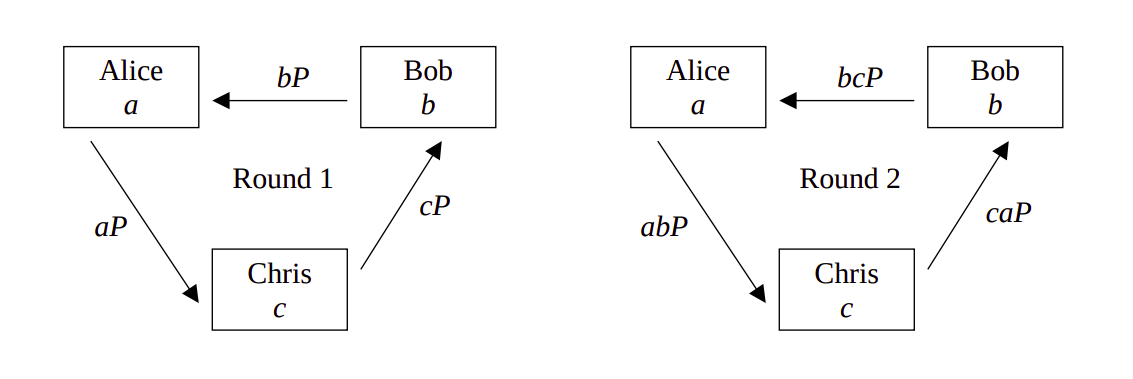
\includegraphics[width=.9\textwidth]{tdhke.png}
	\caption{A two--round three--party key agreement protocol.}
	\label{fig:tdhke}
\end{figure}

The Weil pairing can help us do this in only one round and without requiring any of the three parties to be alive at the same time. The idea is to exploit its bilinearity, so that $e_m(aP, bP)^c = e_m(P, P)^{abc}$. Unfortunately, this na\"{i}ve implementation doesn't work because the Weil pairing is alternating, so $e_m(P, P)^{abc} = 1^{abc} = 1$. However, the idea is quite sound and could be implemented if we had a way to choose two ``independent" points.

\begin{definition}[Distortion map]
    Let $P \in E[m]$, for some prime $m \geq 3$. The map $\phi : E \to E$ is an \textit{$m$--distortion map for $P$} if:
    \begin{enumerate}[label=(\alph*)]
        \item $\phi(nP) = n\phi(P)$
        \item $e_m\left(P, \phi(P)\right)^r = 1 \iff m \;\vert\; r$
    \end{enumerate}
\end{definition}

The following steps describe how the tripartite Diffie--Hellman key exchange works.

\begin{enumerate}[label=\textbf{\arabic*.}]
    \item \textbf{Public parameter creation}: a trusted authority publishes a finite field $\mathbb{F}_q$, an elliptic curve $E/\mathbb{F}_q$, a point $P \in E(\mathbb{F}_q)[m]$ and an $m$--distortion map $\phi$ for $P$.
    \item \textbf{Private computations}:
        \begin{itemize}
            \item Alice chooses a secret integer $n_A$ and computes the point $Q_A = n_A P$
            \item Bob chooses a secret integer $n_B$ and computes the point $Q_B = n_B P$
            \item Chris chooses a secret integer $n_C$ and computes the point $Q_C = n_C P$
        \end{itemize}
    \item \textbf{Public exchange of values}: Alice, Bob and Chris publish their points $Q_A$, $Q_B$ and $Q_C$.
    \item \textbf{Further private computations}: \begin{itemize}
            \item Alice computes $e_m\left(Q_B, \phi\left(Q_C\right)\right)^{n_A}$
            \item Bob computes $e_m\left(Q_A, \phi\left(Q_C\right)\right)^{n_B}$
            \item Chris computes $e_m\left(Q_A, \phi\left(Q_B\right)\right)^{n_C}$
        \end{itemize}
    The final secret value is $e_m\left(P, \phi\left(P\right)\right)^{n_A n_B n_C}$.
\end{enumerate}

The security of this scheme is based off the security of the ECDLP as well as the DLP over $\mathbb{F}_q$. Since sub--exponential algorithms to solve the DLP are known, using tripartite Diffie--Hellman securely requires a larger field than the classical elliptic curve Diffie--Hellman.

\subsubsection{ID--based public key cryptosystems}
When using public key encryption to send a message securely to Alice, Bob encrypts the message using Alice's public key. Alice then uses her corresponding private key to decrypt.

Large--scale deployments of public key cryptography generally employ the services of a certifying authority (CA) who is responsible for generating certificates consisting of Alice's identifying information and her public key, together with the CA's signature on this data. Although the notion of a certificate is very simple, there are many practical difficulties with managing certificates. For example, Bob may not know how to obtain Alice’s certificate. Also, Bob should have the assurance that Alice’s public key is still valid.

In 1984, A. Shamir introduced the notion of identity--based cryptography to alleviate many of the problems inherent with managing certificates. Shamir proposed that Alice's public key consist of her identifying information $\texttt{ID}_A$ (such as Alice's email address). A trusted third party would use its private key to
generate Alice's private key from $\texttt{ID}_A$ and securely transmit it to Alice. Any other party could encrypt messages for Alice using only $\texttt{ID}_A$ and the trusted third party's public key. The first practical identity--based system was devised by D. Boneh and A. Franklin in 2001. This system, which we now describe, uses pairings on elliptic curves.

\begin{enumerate}[label=\textbf{\arabic*.}]
    \item \textbf{Public parameter creation}: a trusted authority, Tom, selects a finite field $\mathbb{F}_q$, an elliptic curve $E$ and a point $P \in E(\mathbb{F}_q)[m]$ of prime order $m$ such that there is an $m$--distortion map $\phi$ for $P$. Tom also publishes two hash functions $H_1 : \{ \text{User ID's} \} \to E(\mathbb{F}_q)$ and $H_2 : \mathbb{F}_q^\ast \to \mathcal{M}$, where $\mathcal{M} = \{0,1\}^B$ is the set of possible plaintexts.
    \item \textbf{Master key creation}: Tom chooses a secret integer $t$ modulo $m$ and publishes $P_T = t P$.
    \item \textbf{Private key extraction}: Alice chooses her ID--based public key $\texttt{ID}_A$ and sends it to Tom. Tom computes and sends to Alice her private key $Q_A = t P_A = t H_1(\texttt{ID}_A)$.
    \item \textbf{Encryption}: Bob chooses a plaintext $M \in \mathcal{M}$ and a random number $r$ modulo $q-1$. He computes $P_A = H_1(\texttt{ID}_A)$ and sends the ciphertext 
    $$\left(C_1, C_2\right) = \left(\; r P, \;\; M \oplus H_2\left(e_m\left(P_A, \phi\left(P_T\right)\right)^r\right) \;\right),$$
    where $\oplus$ denotes the bitwise XOR operation.
    \item \textbf{Decryption}: Alice recovers the plaintext $M$ from $(C_1, C_2)$ by computing 
    $$C_2 \oplus H_2\left(e_m\left(Q_A, \phi\left(C_1\right)\right)\right).$$
\end{enumerate}

The correctness of the decryption step follows from the properties of the XOR operation on bit strings, that is $X \oplus Y \oplus Y = X$ for all bit strings $X,Y$.
\begin{align*}
    C_2 \oplus H_2\left(e_m\left(Q_A, \phi\left(C_1\right)\right)\right) &= \left[M \oplus H_2\left(e_m\left(P_A, \phi\left(P_T\right)\right)^r\right)\right] \oplus H_2\left(e_m\left(Q_A, \phi\left(C_1\right)\right)\right)\\
    &= \left[M \oplus H_2\left(e_m\left(P_A, \phi\left(tP\right)\right)^r\right)\right] \oplus H_2\left(e_m\left(t P_A, \phi\left(rP\right)\right)\right)\\
    &= \left[M \oplus H_2\left(e_m\left(P_A, \phi\left(P\right)\right)^{rt}\right)\right] \oplus H_2\left(e_m\left(P_A, \phi\left(P\right)\right)^{rt}\right)\\
    &= M \oplus \left[H_2\left(e_m\left(P_A, \phi\left(P\right)\right)^{rt}\right) \oplus H_2\left(e_m\left(P_A, \phi\left(P\right)\right)^{rt}\right)\right]\\
    &= M.
\end{align*}

\nocite{*}
\begin{thebibliography}{9}
\bibitem{JH08}
Jeffrey Hoffstein, Jill Pipher, and J.H. Silverman. 2008. \textit{An Introduction to Mathematical Cryptography} (1st. ed.). Springer Publishing Company, Incorporated.
\end{thebibliography}

\end{document}